\documentclass[11pt,a4paper]{article}
\usepackage[T1]{fontenc}
\usepackage[margin=2.3cm]{geometry}
\usepackage{amsmath,amssymb}
\usepackage{graphicx}
\usepackage[dvipsnames]{xcolor}
\usepackage{enumitem}
\usepackage[colorlinks=true,linkcolor=blue,urlcolor=blue]{hyperref}
\setlength{\parskip}{0.6em}
\setlength{\parindent}{0pt}
\begin{document}

\begin{center}{\LARGE\bfseries openstressstrain}\\[0.4em]{\large Read a stress-strain curve and pick a safe material, in three sessions.}\\[0.2em]\small PAN IIT OSS explainer \textbullet{} secondary school to diploma / undergraduate (levels 3-5)\end{center}

\section*{Why this exists}
Every bridge cable, aircraft part and bicycle frame is chosen by how its material stretches and breaks. This explainer shows how a pull test becomes stress, strain, stiffness and yield, and how those numbers pick a size and a material.

\section*{The end goal}
Read a stress-strain curve to pick a safe material. The end goal is to read a stress-strain curve and use it to choose a safe material, as in an engineering materials course. The models here are simplified teaching models with typical values and are not design tools.

\section*{How the three sessions build up}
\begin{enumerate}[nosep]
\item \textbf{Session 1: Pulling a bar: stress, strain and the curve} (Level 1, conceptual interactive model, 60 min).
\item \textbf{Session 2: Hooke's law, strength and a safe design} (Level 2, mathematical engineering model, 75 min).
\item \textbf{Session 3: Elastic-plastic simulation, offset yield and uncertainty} (Level 3, simulation and validation, 90 min).
\end{enumerate}

\section{Session 1: Pulling a bar: stress, strain and the curve}

\subsection*{A. Real-world problem}
A lift cable, a bicycle spoke and a paper clip all get pulled or bent. Pull a paper clip a little and it springs back; pull it hard and it stays bent. How can we describe this with numbers that do not depend on how thick or long the part is? This session uses an illustrative soft metal with round made-up numbers to teach the idea. It is a teaching model, not a design tool, and not data for any real alloy.

\subsection*{B. Concept and theory}
Pull a bar with a force F. The material feels stress: force spread over the cross-section area A. The bar gets longer by an extension dL; dividing by the original length L0 gives strain, which has no unit. A plot of stress against strain is the stress-strain curve, and it describes the material, not the sample. At small stress the bar is elastic: it returns to its original length when you let go, and strain is proportional to stress. Beyond the yield stress it is plastic: it stretches more easily and part of the stretch stays when the load is removed (permanent set).

\begin{itemize}[nosep]
\item F: pulling force (kN)
\item A: cross-section area, pi d\textasciicircum{}2 / 4 for a round bar (mm\textasciicircum{}2)
\item d: bar diameter (mm)
\item sigma: stress = F / A (1 N/mm\textasciicircum{}2 = 1 MPa) (MPa)
\item dL: extension (mm)
\item L0: original length (500 mm here) (mm)
\item eps: strain = dL / L0 (no unit (0.01 is 1 percent))
\item E: stiffness of the illustrative metal (70 000) (MPa)
\item sigma\_y: yield stress of the illustrative metal (200) (MPa)
\end{itemize}

\begin{equation*}
\sigma=\frac{F}{A},\qquad A=\frac{\pi d^2}{4}
\end{equation*}

\begin{equation*}
\varepsilon=\frac{\Delta L}{L_0}
\end{equation*}

\begin{equation*}
\sigma=E\,\varepsilon\quad(\sigma\le\sigma_y),\qquad \varepsilon_{\text{permanent}}=\varepsilon-\frac{\sigma}{E}
\end{equation*}

\begin{center}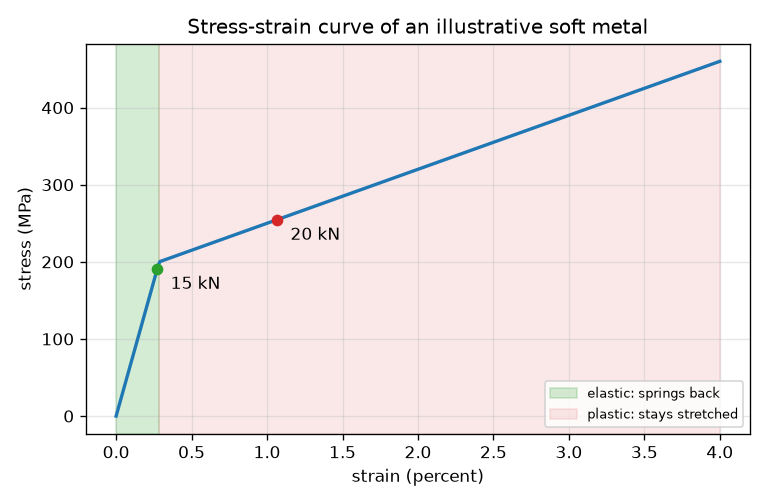
\includegraphics[width=0.85\linewidth]{figures/s01_stress_strain_toy.png}\\\small Stress-strain curve of the illustrative metal with the elastic and plastic regions marked.\end{center}

\subsection*{E. Worked example}
A round bar of diameter 10 mm and length 500 mm is pulled by 15 kN. Find the stress, the strain and the extension, and say whether it is elastic. The yield stress is 200 MPa and E is 70 000 MPa.
\begin{enumerate}[nosep]
\item Area A = pi * 10\textasciicircum{}2 / 4 = 78.54 mm\textasciicircum{}2.
\item Stress = 15 * 1000 N / 78.54 mm\textasciicircum{}2 = 191.0 MPa.
\item 191.0 MPa is below the 200 MPa yield, so the bar is elastic and strain = stress / E = 191.0 / 70 000 = 0.002728.
\item Extension = strain * L0 = 0.002728 * 500 = 1.364 mm.
\item Sanity check: 1.4 mm in 500 mm is a small fraction (0.27 percent), as expected for a stiff metal.
\end{enumerate}
\textbf{Answer.} Stress 191.0 MPa, strain 0.00273, extension 1.36 mm, elastic. At 20 kN the stress is 254.6 MPa, the bar is plastic, the strain is 0.01066 (5.33 mm) and after unloading 0.00703 (3.51 mm) of stretch stays.

\subsection*{F. Questions}
\begin{enumerate}[nosep]
\item \textbf{Conceptual.} Why do engineers plot stress against strain instead of force against extension?
\item \textbf{Numerical.} A bar of diameter 8 mm and length 500 mm is pulled by 10 kN (yield 200 MPa, E = 70 000 MPa). Find the stress, strain and extension. Is it elastic?
\item \textbf{Graph and simulation interpretation.} On the stress-strain curve, at what strain does the curve bend, and how does the slope change there?
\item \textbf{Design and optimisation challenge.} Design: choose the smallest whole-millimetre diameter so that an 18 kN pull keeps the stress at or below 90 percent of the yield stress. State the stress and the extension of your choice.
\end{enumerate}

\section{Session 2: Hooke's law, strength and a safe design}

\subsection*{A. Real-world problem}
A 20 kN load (about 2 tonnes) hangs from a 2 m rod. The rod may stretch by at most 1 mm and must have a factor of safety of 2 against yielding. Which material and which diameter would you choose? This session uses round typical textbook values for four materials. They are for teaching, not design data, and this is not a design tool: real parts also need buckling, joint, fatigue and temperature checks and certified material data.

\subsection*{B. Concept and theory}
In the elastic range stress is proportional to strain: sigma = E eps. E is Young's modulus, the stiffness. Combining sigma = F/A and eps = dL/L gives the extension of a bar: dL = F L / (A E). Yield strength sigma\_y is the stress where permanent stretching starts and ultimate strength sigma\_u is the highest stress on the curve. The factor of safety is yield strength divided by the working stress. A bar must satisfy two limits: strength (stress \textless{}= sigma\_y / FoS gives a minimum area) and stiffness (dL \textless{}= limit gives another minimum area). The larger area governs.

\begin{itemize}[nosep]
\item E: Young's modulus (stiffness) (MPa (1 GPa = 1000 MPa))
\item sigma\_y: yield strength (MPa)
\item sigma\_u: ultimate strength (MPa)
\item rho: density (kg/m\textasciicircum{}3)
\item F: load (20) (kN)
\item L: length (2000) (mm)
\item dL\_max: allowed extension (1.0) (mm)
\item FoS: factor of safety = sigma\_y / sigma (no unit)
\item m: bar mass = rho A L (kg)
\end{itemize}

\begin{equation*}
\sigma=E\,\varepsilon,\qquad \Delta L=\frac{F\,L}{A\,E}
\end{equation*}

\begin{equation*}
\mathrm{FoS}=\frac{\sigma_y}{\sigma},\qquad A\ge\frac{F\,\mathrm{FoS}}{\sigma_y}
\end{equation*}

\begin{equation*}
A\ge\frac{F\,L}{E\,\Delta L_{\max}},\qquad m=\rho\,A\,L
\end{equation*}

\begin{center}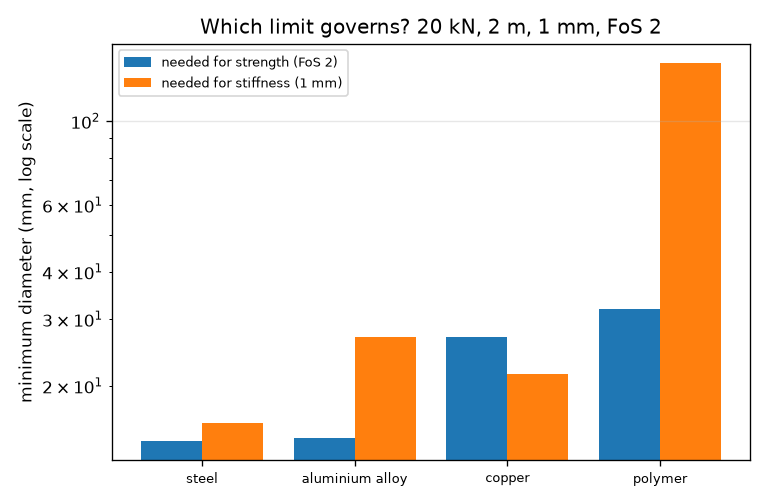
\includegraphics[width=0.85\linewidth]{figures/s02_design_diameters.png}\\\small Minimum diameter for strength and for stiffness of each material (log scale).\end{center}

\subsection*{E. Worked example}
A steel bar (E = 200 000 MPa, yield 250 MPa, density 7850 kg/m\textasciicircum{}3) of length 2 m carries 20 kN. Find the smallest whole-millimetre diameter with FoS \textgreater{}= 2 and extension \textless{}= 1 mm, and check it.
\begin{enumerate}[nosep]
\item Strength: A \textgreater{}= 20 000 * 2 / 250 = 160 mm\textasciicircum{}2, so d \textgreater{}= 14.27 mm.
\item Stiffness: A \textgreater{}= 20 000 * 2000 / (200 000 * 1) = 200 mm\textasciicircum{}2, so d \textgreater{}= 15.96 mm.
\item The larger diameter governs (stiffness), so d = 16 mm (next whole millimetre). A = 201.06 mm\textasciicircum{}2.
\item Check: stress = 20 000 / 201.06 = 99.5 MPa; FoS = 250 / 99.5 = 2.51; extension = 99.5 * 2000 / 200 000 = 0.995 mm.
\item Mass = 7850 * 201.06e-6 * 2 = 3.16 kg.
\end{enumerate}
\textbf{Answer.} d = 16 mm: stress 99.5 MPa, factor of safety 2.51, extension 0.995 mm, mass 3.16 kg. Stiffness governs. Over the four materials the lightest passing bar is the aluminium alloy at d = 27 mm (3.09 kg), only 2 percent lighter than steel, so the choice is sensitive to the data.

\subsection*{F. Questions}
\begin{enumerate}[nosep]
\item \textbf{Conceptual.} Steel and the aluminium alloy in the table have almost the same yield strength, yet the aluminium bar must be much thicker to meet the 1 mm limit. Why?
\item \textbf{Numerical.} An aluminium bar (E = 70 000 MPa, yield 240 MPa) of diameter 27 mm and length 2 m carries 20 kN. Find the stress, the extension and the factor of safety.
\item \textbf{Graph and simulation interpretation.} In the first figure (stress against strain lines), which material is stiffest and which stretches most at its own yield point? Give the strain values.
\item \textbf{Design and optimisation challenge.} Design: the allowed extension is relaxed from 1 mm to 2 mm for the same 20 kN, 2 m, FoS 2. Which of the four materials gives the lightest bar, with a whole-millimetre diameter, and what are its diameter and mass?
\end{enumerate}

\section{Session 3: Elastic-plastic simulation, offset yield and uncertainty}

\subsection*{A. Real-world problem}
Real metals do not have a sharp yield point in a test machine: the curve bends smoothly. So engineers define yield as the stress where a line parallel to the elastic slope, shifted by 0.2 percent strain, crosses the curve. Can we build a model that loads and unloads, find that offset yield numerically, trust it because it matches a hand calculation, and see how much a 10 percent error in the data matters? This is a one-dimensional teaching model with no necking or temperature effects; it is not a validated design tool.

\subsection*{B. Concept and theory}
The Ramberg-Osgood curve adds a power-law plastic strain to Hooke's law: eps = sigma/E + 0.002 (sigma/sigma\_02)\textasciicircum{}n. By construction the plastic part equals 0.002 at sigma = sigma\_02, so sigma\_02 is the 0.2 percent offset yield; n sets how sharp the knee is. The stress for a given strain is found by bisection. Unloading from any point is elastic with the slope E, so the strain left at zero stress is eps\_max - sigma\_max / E. A bilinear metal (slope E, then slope H after yield sigma\_y) is simulated by a return-mapping solver that keeps the plastic strain as a memory. Because inputs are uncertain, sensitivity is the change of an output when one input changes by plus or minus 10 percent.

\begin{itemize}[nosep]
\item E: Young's modulus (MPa)
\item sigma\_02: 0.2 percent offset yield strength (MPa)
\item n: Ramberg-Osgood hardening exponent (no unit)
\item H: slope after yield (bilinear model) (MPa)
\item eps\_p: plastic (permanent) strain (no unit)
\item alpha: accumulated plastic strain (no unit)
\item sigma\_max, eps\_max: peak stress and strain of the loading (MPa, no unit)
\end{itemize}

\begin{equation*}
\varepsilon=\frac{\sigma}{E}+0.002\left(\frac{\sigma}{\sigma_{02}}\right)^{n}
\end{equation*}

\begin{equation*}
\varepsilon_p=\varepsilon_{\max}-\frac{\sigma_{\max}}{E},\qquad \sigma_{\max}=\sigma_y+H\left(\varepsilon_{\max}-\frac{\sigma_y}{E}\right)\ \text{(bilinear)}
\end{equation*}

\begin{equation*}
\sigma_{\text{trial}}=E(\varepsilon-\varepsilon_p),\quad f=|\sigma_{\text{trial}}|-(\sigma_y+H_p\alpha),\quad \Delta\gamma=\frac{f}{E+H_p},\quad H_p=\frac{EH}{E-H}
\end{equation*}

\begin{center}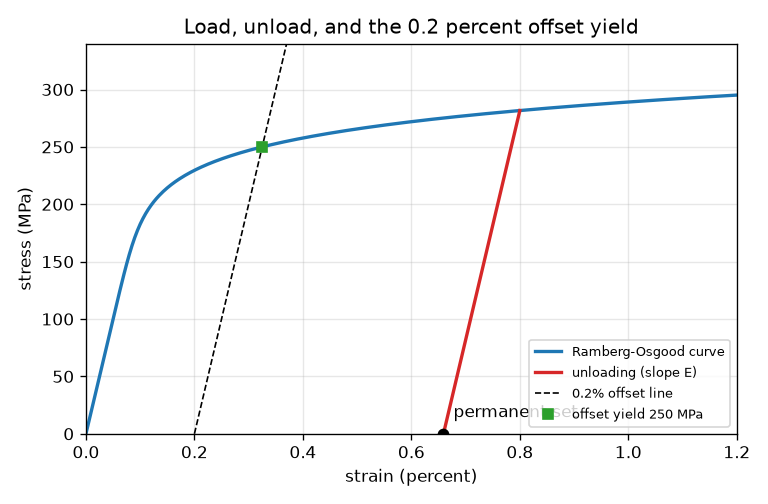
\includegraphics[width=0.85\linewidth]{figures/s03_load_unload.png}\\\small Ramberg-Osgood curve loaded to 0.8 percent strain, the elastic unloading line, the permanent set and the 0.2 percent offset yield.\end{center}

\subsection*{E. Worked example}
A bilinear metal has E = 70 000 MPa, yield 200 MPa and slope H = 7 000 MPa after yield. It is pulled to 2 percent strain and then unloaded. Find the peak stress and the permanent set, and compare with the solver.
\begin{enumerate}[nosep]
\item Yield strain = 200 / 70 000 = 0.002857.
\item Peak stress = 200 + 7000 * (0.02 - 0.002857) = 200 + 120 = 320 MPa.
\item Unloading is elastic, so the elastic strain recovered is 320 / 70 000 = 0.004571.
\item Permanent set = 0.02 - 0.004571 = 0.015429 (1.54 percent).
\item The return-mapping solver gives 320.00 MPa at the top and zero stress at strain 0.01543: it matches the hand calculation.
\end{enumerate}
\textbf{Answer.} Peak stress 320 MPa; permanent set 0.01543 (1.54 percent). The solver reproduces both.

\subsection*{F. Questions}
\begin{enumerate}[nosep]
\item \textbf{Conceptual.} Why do engineers use the 0.2 percent offset yield instead of the point where the curve first leaves the straight line?
\item \textbf{Numerical.} A bilinear metal with E = 70 000 MPa, yield 200 MPa and H = 7 000 MPa is pulled to 1 percent strain and unloaded. Find the peak stress and the permanent set.
\item \textbf{Graph and simulation interpretation.} Read the sensitivity table for the steel bar (20 kN, 2 m, d = 16 mm). Which input matters for the stretch and which for the safety factor, and by how much for a 10 percent change?
\item \textbf{Design and optimisation challenge.} Design: the steel bar must still stretch no more than 1 mm if the real E is 10 percent below the table (180 GPa) and must keep FoS \textgreater{}= 2 if the real yield is 10 percent low (225 MPa). Choose the smallest whole-millimetre diameter and compare its mass with the 16 mm bar.
\end{enumerate}

\section{Real-world mini-project}
\textbf{Estimate E and yield from a noisy tensile test.} A lab hands you stress-strain readings from a tensile test, but the readings are noisy. In this project the data is generated in code (\texttt{synthetic\_test} in Session 3) from a hidden material, so you can check your answer. Choose the strain or stress window for the straight-line fit of E, then find the 0.2 percent offset yield with \texttt{offset\_yield}. Repeat for 50 random seeds with \texttt{noise\_mpa=5.0} and report the mean and spread.

\section{The path ahead}
\begin{enumerate}[nosep]
\item \textbf{Session 4: True stress, true strain and necking.} A converter from engineering to true stress and strain and a detector of the necking point on a power-law hardening metal.
\item \textbf{Session 5: Fit the whole curve with uncertainty.} A fitting script with a chosen fit window and a bootstrap estimate of the spread.
\item \textbf{Session 6: Material selection by strength per density.} A table and an Ashby-style log-log chart of yield strength against density with a guide line.
\item \textbf{Session 7: Probability of failure by Monte Carlo.} A sampler that draws yield from a normal distribution and reports the failure probability.
\item \textbf{Session 8: Reproduce the Target: tensile test with necking and a selection chart.} An animated specimen, a live engineering curve and a log-log chart.
\end{enumerate}

\section{Answers and hints}

\subsection*{Session 1}
\begin{enumerate}[nosep]
\item \textbf{Conceptual.} Hint: Think of a thick bar and a thin bar of the same metal. Do they need the same force to break? Solution: A thick bar needs a larger force than a thin bar to reach the same damage, and a long bar stretches more than a short one. Dividing the force by the area and the extension by the length removes the size of the sample, so one curve describes the material and can be used for any size.
\item \textbf{Numerical.} Hint: A = pi d\textasciicircum{}2 / 4 first, then stress = F / A. Solution: A = pi * 8\textasciicircum{}2 / 4 = 50.27 mm\textasciicircum{}2. Stress = 10 000 / 50.27 = 198.9 MPa. This is just below the 200 MPa yield, so the bar is elastic. Strain = 198.9 / 70 000 = 0.002842 and extension = 0.002842 * 500 = 1.42 mm. Units: MPa, no unit, mm. Sanity check: the stress is close to yield, so the bar is almost at its limit.
\item \textbf{Graph and simulation interpretation.} Hint: Strain at yield = yield stress / E. The slope after yield is 7 000 MPa. Solution: The bend is at strain 200 / 70 000 = 0.00286 (0.29 percent). Before it the slope is E = 70 000 MPa; after it the slope is 7 000 MPa, ten times flatter. A flatter curve means the metal needs much less extra stress to stretch further, and the stretch is no longer recoverable.
\item \textbf{Design and optimisation challenge.} Hint: The allowed stress is 0.9 * 200 = 180 MPa, so A must be at least F divided by that. Solution: A \textgreater{}= 18 000 / 180 = 100 mm\textasciicircum{}2, so d \textgreater{}= sqrt(4 * 100 / pi) = 11.28 mm; the smallest whole millimetre is 12 mm. Check: A = 113.1 mm\textasciicircum{}2, stress = 159.2 MPa (about 80 percent of yield), strain = 0.002274 and extension = 1.14 mm. d = 11 mm would give 189.4 MPa, too close to yield. Trade-off: a thicker bar is safer but heavier and costlier.
\end{enumerate}

\subsection*{Session 2}
\begin{enumerate}[nosep]
\item \textbf{Conceptual.} Hint: Which property controls how much a bar stretches, strength or stiffness? Solution: The extension depends on E, the stiffness, not on the yield strength. Aluminium has about a third of the stiffness of steel (70 against 200 GPa), so for the same load it stretches nearly three times as much unless its area is larger. Strength only decides when the metal yields.
\item \textbf{Numerical.} Hint: A = pi d\textasciicircum{}2 / 4; stress = F / A; dL = stress * L / E; FoS = yield / stress. Solution: A = 572.56 mm\textasciicircum{}2. Stress = 20 000 / 572.56 = 34.93 MPa. Extension = 34.93 * 2000 / 70 000 = 0.998 mm, just inside the 1 mm limit. FoS = 240 / 34.93 = 6.87. Sanity check: the factor of safety is far above 2 because the stretch limit, not strength, sized the bar.
\item \textbf{Graph and simulation interpretation.} Hint: The slope is E; the strain at yield is yield / E. Solution: Steel has the steepest line (E = 200 GPa). Strain at yield: steel 250 / 200 000 = 0.00125 (0.125 percent); aluminium 0.00343; copper 0.00064; the polymer 50 / 2500 = 0.02 (2 percent), the largest. The polymer is the least stiff and stretches most before yield, even though its yield stress is the lowest.
\item \textbf{Design and optimisation challenge.} Hint: Compute both minimum diameters for each material (use \texttt{best\_design(dl\_max=2.0)}), take the larger, round up and compare masses. Solution: Aluminium alloy: strength d \textgreater{}= 14.57 mm, stiffness d \textgreater{}= 19.07 mm, so d = 20 mm, mass 1.70 kg, extension 1.82 mm, FoS 3.77. Steel: stiffness 11.28 mm, strength 14.27 mm (strength now governs), d = 15 mm, mass 2.77 kg. Copper needs 27 mm (10.19 kg) and the polymer 101 mm (18.43 kg). The aluminium alloy is lightest. Trade-off: a looser stretch limit makes the lighter, less stiff material attractive; cost, joining and the scatter of real material data also matter.
\end{enumerate}

\subsection*{Session 3}
\begin{enumerate}[nosep]
\item \textbf{Conceptual.} Hint: Can you see exactly where a smooth curve leaves its tangent line? Solution: A smooth curve departs from its straight part gradually, so the 'first point of departure' depends on how closely you look and on noise. The offset construction gives a well-defined, repeatable number that any lab can find from the same data, at the price of choosing 0.2 percent by convention. It means the metal has a permanent set of about 0.2 percent when unloaded at that stress.
\item \textbf{Numerical.} Hint: Peak stress = yield + H (eps - yield/E). Permanent set = eps - peak / E. Solution: Yield strain = 0.002857. Peak stress = 200 + 7000 * (0.01 - 0.002857) = 250.0 MPa. Permanent set = 0.01 - 250 / 70 000 = 0.006429 (0.64 percent). Units: MPa and no unit. Sanity check: the set must be less than the total strain 0.01.
\item \textbf{Graph and simulation interpretation.} Hint: Extension is proportional to 1/E and the factor of safety to the yield strength. Solution: E -10 percent raises the extension by 11.1 percent (1/0.9 - 1) and E +10 percent lowers it by 9.1 percent; the factor of safety does not depend on E. Yield -10 percent lowers the factor of safety by exactly 10 percent (2.51 to 2.26) and the extension does not depend on yield. So stiffness data controls the stretch check and yield data controls the safety check.
\item \textbf{Design and optimisation challenge.} Hint: Use worst-case E and yield in the formulas of Session 2 (\texttt{bar\_response(180000, 225, d\_mm=...)}). Solution: Stiffness: A \textgreater{}= 20 000 * 2000 / (180 000 * 1) = 222.2 mm\textasciicircum{}2, so d \textgreater{}= 16.82 mm, which is 17 mm. At 17 mm: extension 0.979 mm and FoS 2.55 (with yield 225 MPa), so both limits pass. The 16 mm bar would stretch 1.105 mm in the worst case. Mass of 17 mm: 3.56 kg against 3.16 kg for 16 mm. Trade-off: robustness against data uncertainty costs about 13 percent more material.
\end{enumerate}

\section{How to join}
Read \texttt{CONTRIBUTING.md} in the repository, then pick an issue labelled \texttt{good first issue}. Repository: \url{https://github.com/KrunalPanchal1995/openstressstrain}

\end{document}
